\subsection{LINQ}
\label{sec:linq}

\epigraph{The code regions which take the most execution time are called \textit{hot spots}. The hot spots are the best places to tune and optimize because a little bit of effort on making a hot spot faster can have a big pay-off. It’s not worth spending engineering effort on a bit of code that executes only once or doesn’t take much time.}
{\textit{Paul J. Drongowski \\ \footnotesize{PERF tutorial: Finding execution hot spots\protect\footnotemark}}}

\footnotetext{http://sandsoftwaresound.net/perf/perf-tutorial-hot-spots/}

An explicit performance consideration mentioned in the "Contributing Code" guidelines on the project's Github page\footnote{\url{https://roslyn.codeplex.com/wikipage?title=How\%20to\%20Contribute}} explicitly mentions \gls{linq}\footnote{LINQ: Language-Integrated Query, syntax features to query data}:

\begin{quote}
Avoid allocations in \gls{compiler} hot paths:
\begin{itemize}
\item Avoid \gls{linq}.
\item Avoid using \texttt{foreach} over collections that do not have a \texttt{struct} enumerator.
\item Consider using an object pool. There are many usages of object pools in the \gls{compiler} to see an example.
\end{itemize}
\end{quote}

It's already clear that the main idea here is minimizing allocations made -- an overarching theme which we have also discussed in previous sections. In this section we will focus on \gls{linq} and some of the performance implications that come with it. The two other bullet points also have to do with memory allocation: both concern memory allocation on the heap which will eventually trigger a \gls{gc}.

The concern here is that \gls{linq} adds an unacceptable overhead in the team's eyes. This overhead is inherent to \gls{linq}: you make a trade-off between memory and performance impact and instead end up with much more readable code. 

As means of a simple test, we'll take a look at a snippet of code and its \gls{linq} alternative and compare their memory impact. We'll create two memory snapshots and see how many extra objects have been created for each implementation. It should obviously be noted that not all \gls{linq} statements are equally wasteful and in some scenarios \gls{linq} can even make sure there is less memory impact.

The code we use to test can be found in listing \ref{lst:linq-memory} and adds 3 items from one list to another based on a certain condition. One approach uses a \gls{linq} query while the other uses a \texttt{foreach} loop which is basically the unrolled equivalent of the former. The heap snapshots in figures \ref{img:performance-linq-memlinq} and \ref{img:performance-linq-memloop} give use a clear view of what objects are being allocated along the way: we can see that constructing the \gls{linq} query creates two new objects of types \texttt{Enumerable+WhereListIterator<Int32>} and \texttt{Func<Int32, Boolean>}, representing the \texttt{Where} structure and the where condition respectively. Additionally there is an object \texttt{HandleCollector+HandleType} which is overhead created by the \glslink{gc}{GC}. 

When we take a look at the next snapshot we can see that after Garbage Collecting and running our \texttt{foreach} loop, we now notice that we only create the overhead object and that the \texttt{WhereListIterator} has been Garbage Collected. You might wonder what happened to the \texttt{Func} -- in the end, that condition isn't referenced anywhere anymore and as such it should be eligible for collection. The optimization at play here is that the \gls{compiler} caches lambdas if they adhere to certain characteristics such as not using a local variable\footnote{http://stackoverflow.com/a/6280711/1864167}. By using this lambda in our code we now have an object that will live for a long time and, by definition, increase memory pressure. Using the caching technique keeps this memory pressure limited but knowing that there are at least one or two object allocations for the simplest of \gls{linq} queries makes it easy to see why they should be avoided in hot paths.


\begin{figure}
\centering
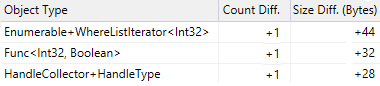
\includegraphics[scale=1]{performance-linq-memlinq}
\caption{Memory impact when comparing the LINQ query to the baseline}
\label{img:performance-linq-memlinq}
\end{figure}

\begin{figure}[h]
\centering
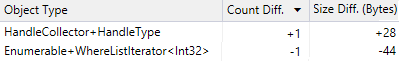
\includegraphics[scale=1]{performance-linq-memloop}
\caption{Memory impact when comparing the loop to the LINQ query}
\label{img:performance-linq-memloop}
\end{figure}

\lstset{style=csharp, caption={Comparing LINQ memory impact}}
\begin{lstlisting}[label={lst:linq-memory}]
static void Main(string[] args)
{
    // Setting baseline snapshot
    var list1 = new List<int> {4862, 6541, 7841};
    var list2 = new List<int>(list1.Count);
    var list3 = new List<int>(list1.Count);

    // First snapshot: LINQ usage
    list2.AddRange(list1.Where(item => item > 5000 && 
																			 item < 7000));

    // Second snapshot: foreach-loop
    foreach (var item in list1)
    {
        if (item > 5000 && item < 7000)
        {
            list3.Add(item);
        }
    }
}
\end{lstlisting}
